\documentclass{article}

\usepackage{amsmath, amsthm, amssymb, amsfonts}
\usepackage{thmtools}
\usepackage{graphicx}
\usepackage{setspace}
\usepackage{geometry}
\usepackage{float}
\usepackage{hyperref}
\usepackage[utf8]{inputenc}
\usepackage[english]{babel}
\usepackage{framed}
\usepackage[dvipsnames]{xcolor}
\usepackage{tcolorbox}
\usepackage{tikz}
\usepackage{booktabs}
\usepackage{tabularray}
\usepackage{algorithm}
\usepackage{algpseudocode}

\colorlet{LightGray}{White!90!Periwinkle}
\colorlet{LightOrange}{Orange!15}
\colorlet{LightGreen}{Green!15}

\newcommand{\HRule}[1]{\rule{\linewidth}{#1}}

\declaretheoremstyle[name=Theorem,]{thmsty}
\declaretheorem[style=thmsty,numberwithin=section]{theorem}
\tcolorboxenvironment{theorem}{colback=LightGray}

\declaretheoremstyle[name=Proposition,]{prosty}
\declaretheorem[style=prosty,numberlike=theorem]{proposition}
\tcolorboxenvironment{proposition}{colback=LightOrange}

\declaretheoremstyle[name=Principle,]{prcpsty}
\declaretheorem[style=prcpsty,numberlike=theorem]{principle}
\tcolorboxenvironment{principle}{colback=LightGreen}

\setstretch{1.2}
\geometry{
	textheight=9in,
	textwidth=5.5in,
	top=1in,
	headheight=12pt,
	headsep=25pt,
	footskip=30pt
}


\tikzstyle{terminator} = [rectangle,draw,text centered, rounded corners, minimum height=2em, minimum width=2em, draw=black, fill=red]

\tikzstyle{data}=[rectangle, draw, text centered, minimum height=2em, draw=black, fill=blue]

\tikzstyle{process} = [rectangle, draw, minimum height=1em, 
minimum width=3em, text centered, draw=black, fill=orange]

\tikzstyle{decision} = [diamond, draw, text centered, minimum height=1em, 
minimum width=3em, draw=black, fill=green]

% ------------------------------------------------------------------------------

\begin{document}
	
	% ------------------------------------------------------------------------------
	% Cover Page and ToC
	% ------------------------------------------------------------------------------
	
	\title{ \normalsize \textsc{}
		\\ [2.0cm]
		\HRule{1.5pt} \\
		\LARGE \textbf{\uppercase{Peaky Finders}
			\HRule{2.0pt} \\ [0.6cm] \LARGE{EEG Peak Prediction} \vspace*{10\baselineskip}}
	}
	\date{}
	\author{\textbf{Author} \\ 
		Xinyu Qian and Satyarth Arora \\
		March 5, 2025}
	
	\maketitle
	\newpage
	
	\tableofcontents
	\newpage
	
	% ------------------------------------------------------------------------------
	\section{Abstract}
	This paper proposes a peak detection algorithm/model to recognize and label specific peaks found in an EEG signal. The model uses audiovisual interaction EEG data collected in Dr. Ozdamar's lab supplemented with EEG data found in online public databases.
	
	\section{Plan}
	\subsection{Peaks in an EEG signal}
	Our first plan of action is to extrapolate and explain in the most simplest terms, the different peaks observed in an EEG signal. We also will expand on meta properties about the peaks which will feed in to our algorithm as features.
	
	\subsection{Experiment Biases}
	As compositions of EEG signals are dependent on
	\begin{itemize}
		\item Equipment Setup: Type and number of electrodes used to record the data.
		\item Experiment Setup: Which part of the human brain is targeted for the experiment.
	\end{itemize}
	
	We will be describing the biases and providing justification on how our algorithm is bias independent/dependent.
	
	\subsection{Labeling and Validation of Peaks}
	
	To verify whether the peaks we are trying to find are accurate, we will be validating our EEG peak database from a domain expert (Dr. Ozdamar).
	
	\subsection{Strategies for Isolating Peaks}
	Next step is researching the state of the art on Isolation and peak extraction using signal processing or ML approaches.
	
	\subsection{Model/Algorithm Proposal}
	
	Upon doing the above, we will propose an architecture describing the best process (in our opinion) to achieve peak extraction and labelling.
	
	

		
	
	
	\newpage
	
	\section{Visual Evoked Potential Peaks\cite{becker2005visual}}
	
	\subsection{N35}
	N35 are peaks observed at around 35 ms post stimulus. They are recorded over the occipital or parietal regions. Observations have shown that this peak originates from the primary visual cortex (V1) and possibily extrastriate areas, reflecting the initial cortical response. It is inflenced by low-level visual features. (What Features?)
	
	\subsection{P50}
	P50 are peaks observed at 45-60 ms post stimulus, produced by retinal ganglion cells and other retinal cellular elements, V1 is also involved. It is sensitive to stimulus features, the amplitude can be modulated by attention and stimulus saliency (frontal lobe involved).
	
	
	\subsection{N75}
	N75 are early negative peaks observed at around 75 ms post stimulus, a hallmark component of the pattern-reversal VEP, most prominent over the occipital cortex, often followed by P100. It is associated with the initial cortical response to visual contrast and pattern detection. It is also linked to the parvocellular pathway.
	
	\subsection{P100}
	P100 is a large positive peak observed at 80-130 ms post stimulus. P100 is a prominent peak that is used for analysis, as it has relatively little variation between subjections, minimal within subject interocular difference, and minimal variation with repeated measurement over time. P100 peak time is affected by nonpathophyiologic parameters such as pattern size, pattern contrast, mean luminence, signal filtering, patient age, refractive error, poor fixation and miosis.
	
	\subsection{N170}
	N170 is a negative peak around 140-180 ms, typically at ~170 ms post stimulus, most prominent over the occipitotemporal regions. N170 is strongly associated with face perception but also responds to other complex visual objects. Examples include words, cars in experts. Primarily generated in the fusiform gyrus (FG, part of the fusiform face area, FFA) and superior temporal sulcus (STS).
	
	\subsection{P200}
	P200 is a positive peak observed at 180-250 ms post stimulus. Most prominent over frontal, central and parietal electrodes, but can also appear in occipitotemporal regions, depending on stimulus type. It is associated with higher order visual processing, including feature detection, attention allocation and stimulus categorization. Modulated by top-down attention and expectation.
	
	\subsection{P3}
	This is a positive peak observed at 250-500 ms. This is an important VEP peak. It is most prominent over the parietal and central regions, often visible at Pz and Cz sites. It reflects higher-order cognitive processing, particularly stimulus evaluation, decision-making and memory updating. It is most commonly observed in oddball paradigms. P3 amplitude is influenced by task difficulty, stimulus salience and attention. Larger P3 amplitudes are typically seen for attended or relevant stimuli. The latency of P3 is often used as an index of cognitive processing speed and is reflected by stimulus complexity and cognitive load.
	
	\section{Peaks for Auditory\cite{lightfoot2016summary}}
	\subsection{N0}
	Its an early negative peak \textcolor{red}{(Latency needs to be found)}. It is observed primarily over the vertex (Cz) and frontocentral regions, with contributions from temporal electrodes. It is likely generated by thalamic and primary auditory cortex activity. Sensitive to stimulus features such as intensity and frequency.
	
	\subsection{P1}
	This is an early positive peak observed at 50-100 ms post stimulus in adults (Earlier in children). It is maximal over frontocentral regions (Cz, Fz) and sometimes detected at temporal sites. P1 reflects early cortical processing of auditory stimuli, including sound detection and encoding. They are generated mainly in the primary auditory cortex with contributions from secondary auditory areas.
	
	\subsection{N1}
	This is a negative peak observed at 100 ms post stimulus. N1 reflects cortical processing of auditory stimuli, likely generated in the primary auditory cortex (A1) and secondary auditory areas. The amplitude and latency of N1 are modulated by attention, sound saliency and stimulus relevance.
	
	\subsection{P2}
	This is a positive peak observed at 150-200 ms post stimulus. P2 reflects further cortical processing of auditory stimuli, especially in terms of sound discrimination, attention and categorization. It is generated primarily in the secondary auditory cortex, but can involve other regions such as the prefrontal cortex and parietal areas, depending on the attentional demands of the task. Amplitude of P2 is modulated by stimulus saliency and attentional focus.
	
	\subsection{N2}
	This is a negative peak observed at 170-250 ms post stimulus. It is most prominent over frontocentral and central regions (Cz, Fz, Pz). N2 reflects higher-order auditory processing, involving cognitive and attentional mechanisms. It is particularly associated with the cognitive control of auditory attention and the detection of target stimuli in oddball paradigms. The amplitude of N2 is modulated by the saliency of the auditory stimulus.
	
	
	\section{Dataset}
	\subsection{Theory}
	Sound-Induced Flash Illusion (SIFI) has become a valuable tool for investigating audiovisual (AV) processing in the brain. SIFI demonstrated that sound can influence visual perception, similar to how visual lipreading alters auditory perception in AV speech. Previously, the popular view among scholars was that information-processing circuits for different senses operate independently within the brain up to the cortex and vision dominates other senses (two ref). However, SIFI and other instances of multisensory interaction suggest that auditory dominates in some instances of SIFI. When different types of stimulation occur at the same time, there may be neural components in the brain associated with multi-sensory interaction.
	
	\subsection{Equipment Setup}
	Two-channel electrode montages were placed on the subject's head to collect auditory and visual EEG signals. The auditory channel is composed of $C_z$ as the positive electrode, with the right and left mastoids (linked) as the negative electrode. It collects signals from the ear(Ear receives tone stimuli) to the auditory cortex (which processes auditory perception).
	
	The visual channel consists of $O_z$ as the positive elctrode and $F_z$ as the negative electrode. It collects signals from the eyes (which receive flash stimuli) to the visual cortex in the occipital lobe (which processes visual perception). $F_{pz}$ serves as the common ground electrode for both audio and visual channels to reduce the interference of external noise with the experiment.
	
	\subsection{Recording Process}
	SmartEP software by IHS is used to record the EEG signal in real-time. The SIFI program was configured in SmartEP data collection software to present subjects with nine random combinations of flash and beep stimuli (0,1, or 2 times for one short routine), asking them to identify the stimuli they perceive. EEG data were collected during each trial, with a total of 256 sweeps (Poking the brain) with a sampling rate of 8000Hz or a sample is recorded every 125us. A 600 ms signal was recorded.
	
	\section{Plot Visualization}
	The samples recovered from the SmartEP software is a 1-D time series vector. The length of each vector is 4096 which is equivalent to 600 ms (Sampling Rate = 8000 Hz). The SmartEP software also exported out the position (ms) of the manually annotated labels for the peaks which we were able to utilize to create our plot functions. The dataset exported from Dr Ozdamar's lab was incomplete as for some time vectors, peaks were labelled and for some they were not. Due to the malformed dataset, we couldn't explore any supervised machine learning methods for automated peak detection and labelling. Therefore we explored signal processing techniques and came up with algorithms for certain peaks.
	\section{Methods}
	To design the algorithms, we looked at existing literature to see if we can find out any statistical features or properties that can provide a heuristic for the algorithms. The only feature we could find is time window analysis which are summarized in Table \ref{tbl:VEP_TimeWindow} and \ref{tbl:AEP_TimeWindow}.
	
	\subsection{P100 Detection Algorithm}
	\begin{algorithm}
		\caption{P100 Detection Algorithm}\label{alg:P100Algorithm}
		\begin{algorithmic}
			\Require $size(x) \geq 4096 \approxeq 600ms$
			\State $x = x[80/8000 : 130/8000]$
			\For{i = 2 to size(x)}
				\State $y = x[i] - x[i-1]$			
			\EndFor
			\For{i = 1 to size(y)}
				\If{$y[i] > 0$}
					\State $z.pushBack(y[i])$
				\EndIf
			\EndFor
			\State $maxPeak = z[0]$
			\For{i = 2 to size(z)}
				\If{$maxPeak < z[i]$}
					\State $maxPeak = z[i]$
				\EndIf
			\EndFor
			\State $index = 0$
			\For{i = 1 to size(x)}
				\If{$maxPeak == x[i]$}
					\State $index = i$
				\EndIf
			\EndFor
			\\
			\Return $i*8000/4096$
			
		\end{algorithmic}
	\end{algorithm}
	
	
	\subsection{Observation}
	From comparing the P100 Labels with the ones detected by the algorithm, we saw that the dataset has errors in labelling which is due to the limitation of the SmartEP software. Errors such as the labels not part of the time series vector.
	The plot and errors are showcased in Fig. ~\ref{LF-SIFI-1} and ~\ref{LF-SIFI-1-Error}. We then used the algorithm to label the time series vector. The P100 label from the dataset and the one determined by the algorithm is shown in Fig. ~\ref{LF-SIFI-1-ErrorFix}.
	
	
	\begin{figure}[tbh!]\label{LF-SIFI-1}
		\centering
		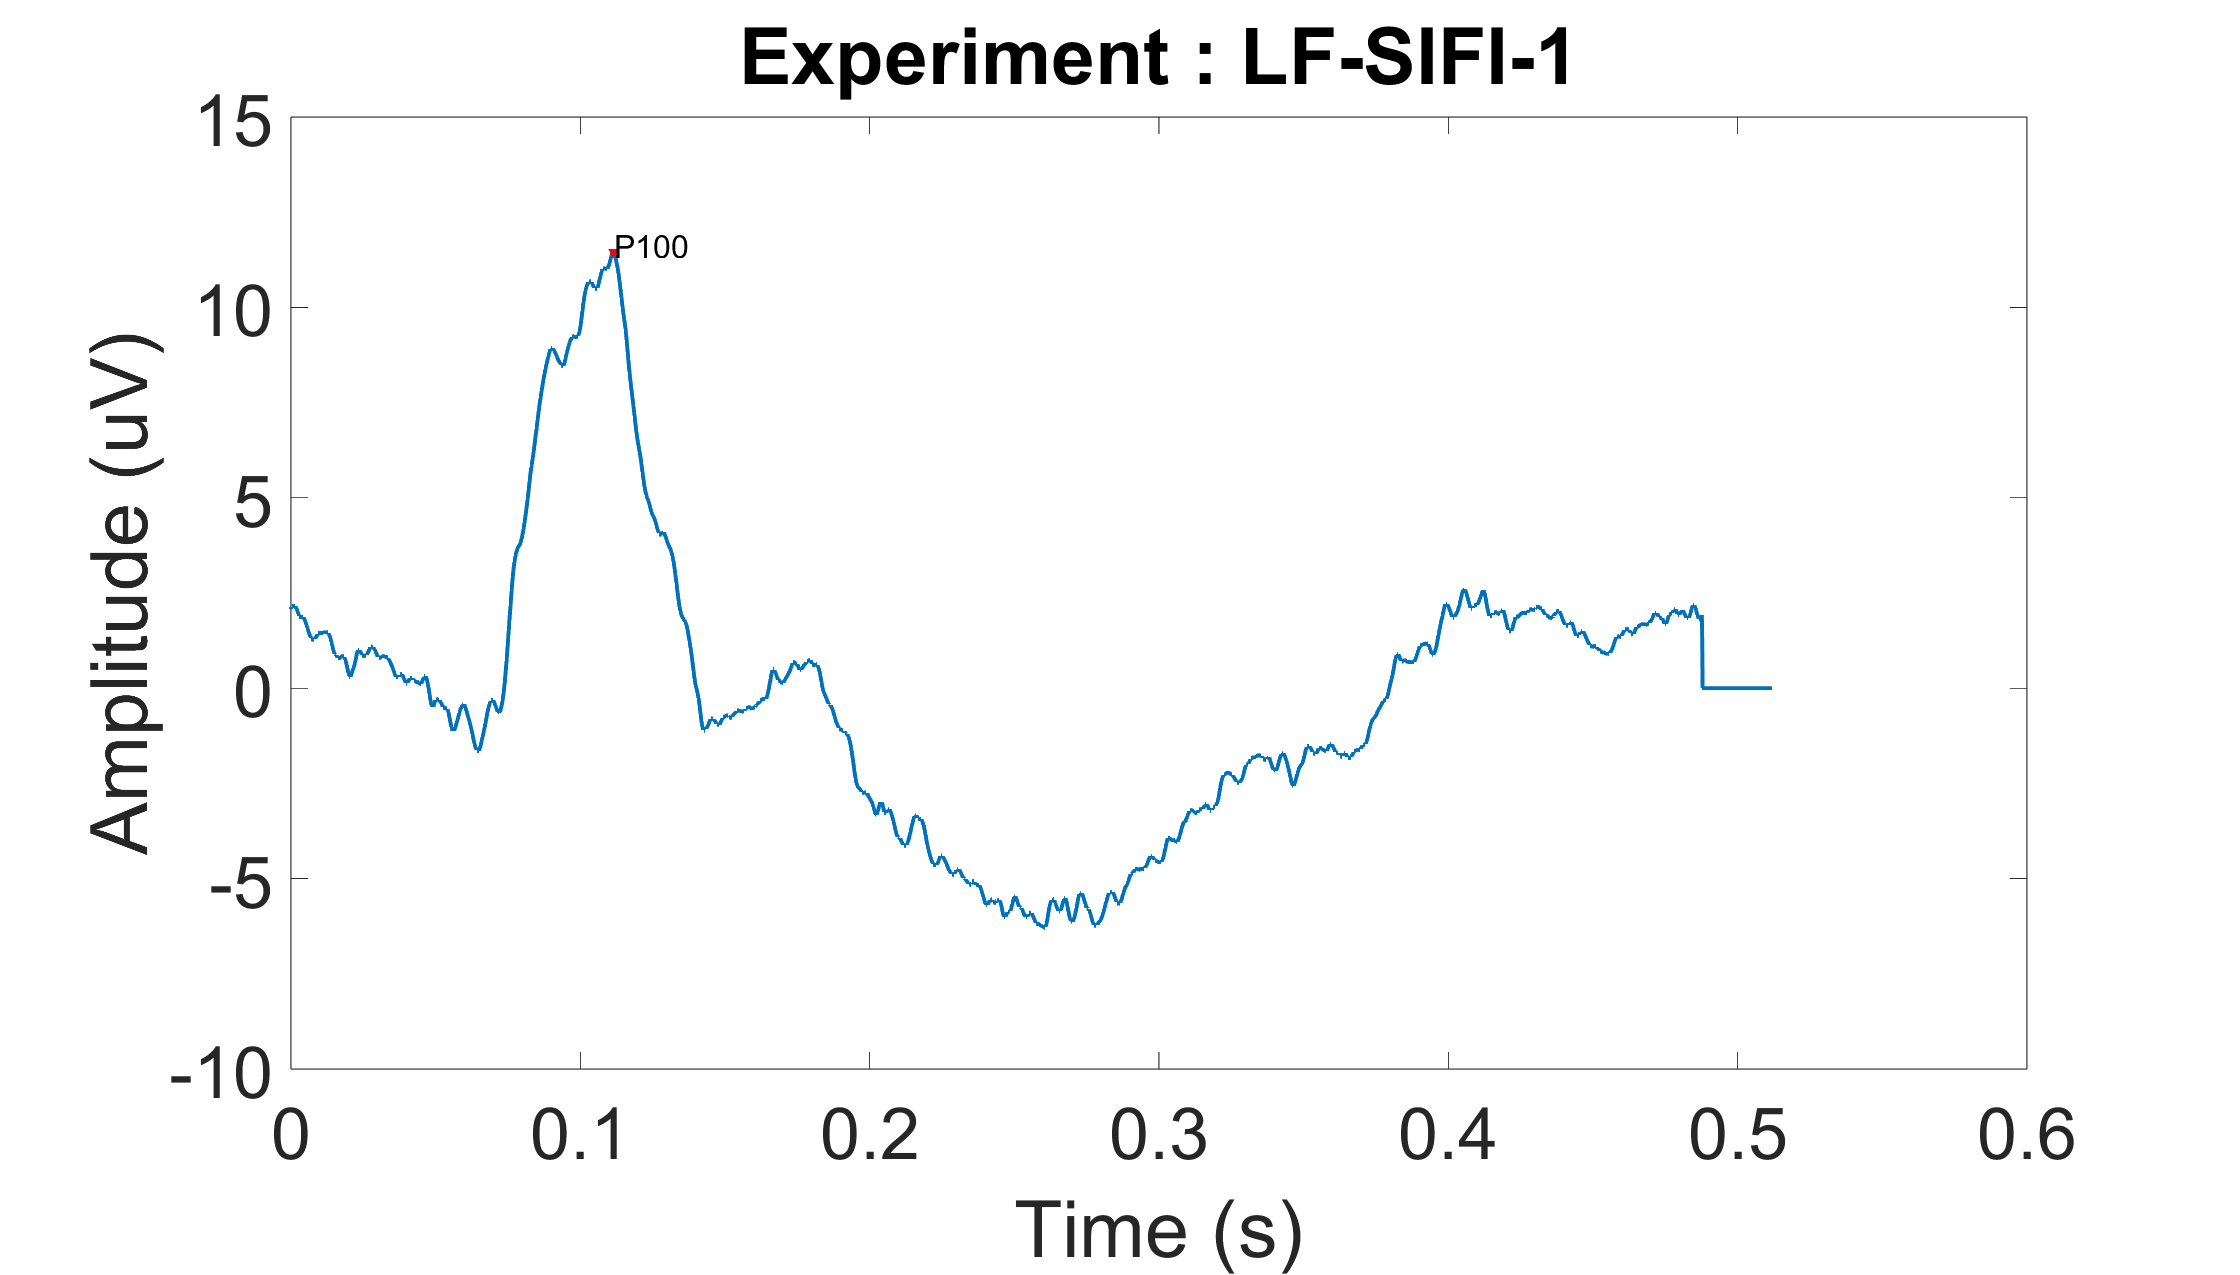
\includegraphics[scale=0.2]{"Images/LF-SIFI-1_Plot.png"}
		\caption{P100 Label | LF-SIFI-1 (Dataset)}
	\end{figure}
	
	\begin{figure}[tbh!]\label{LF-SIFI-1-Error}
		\centering
		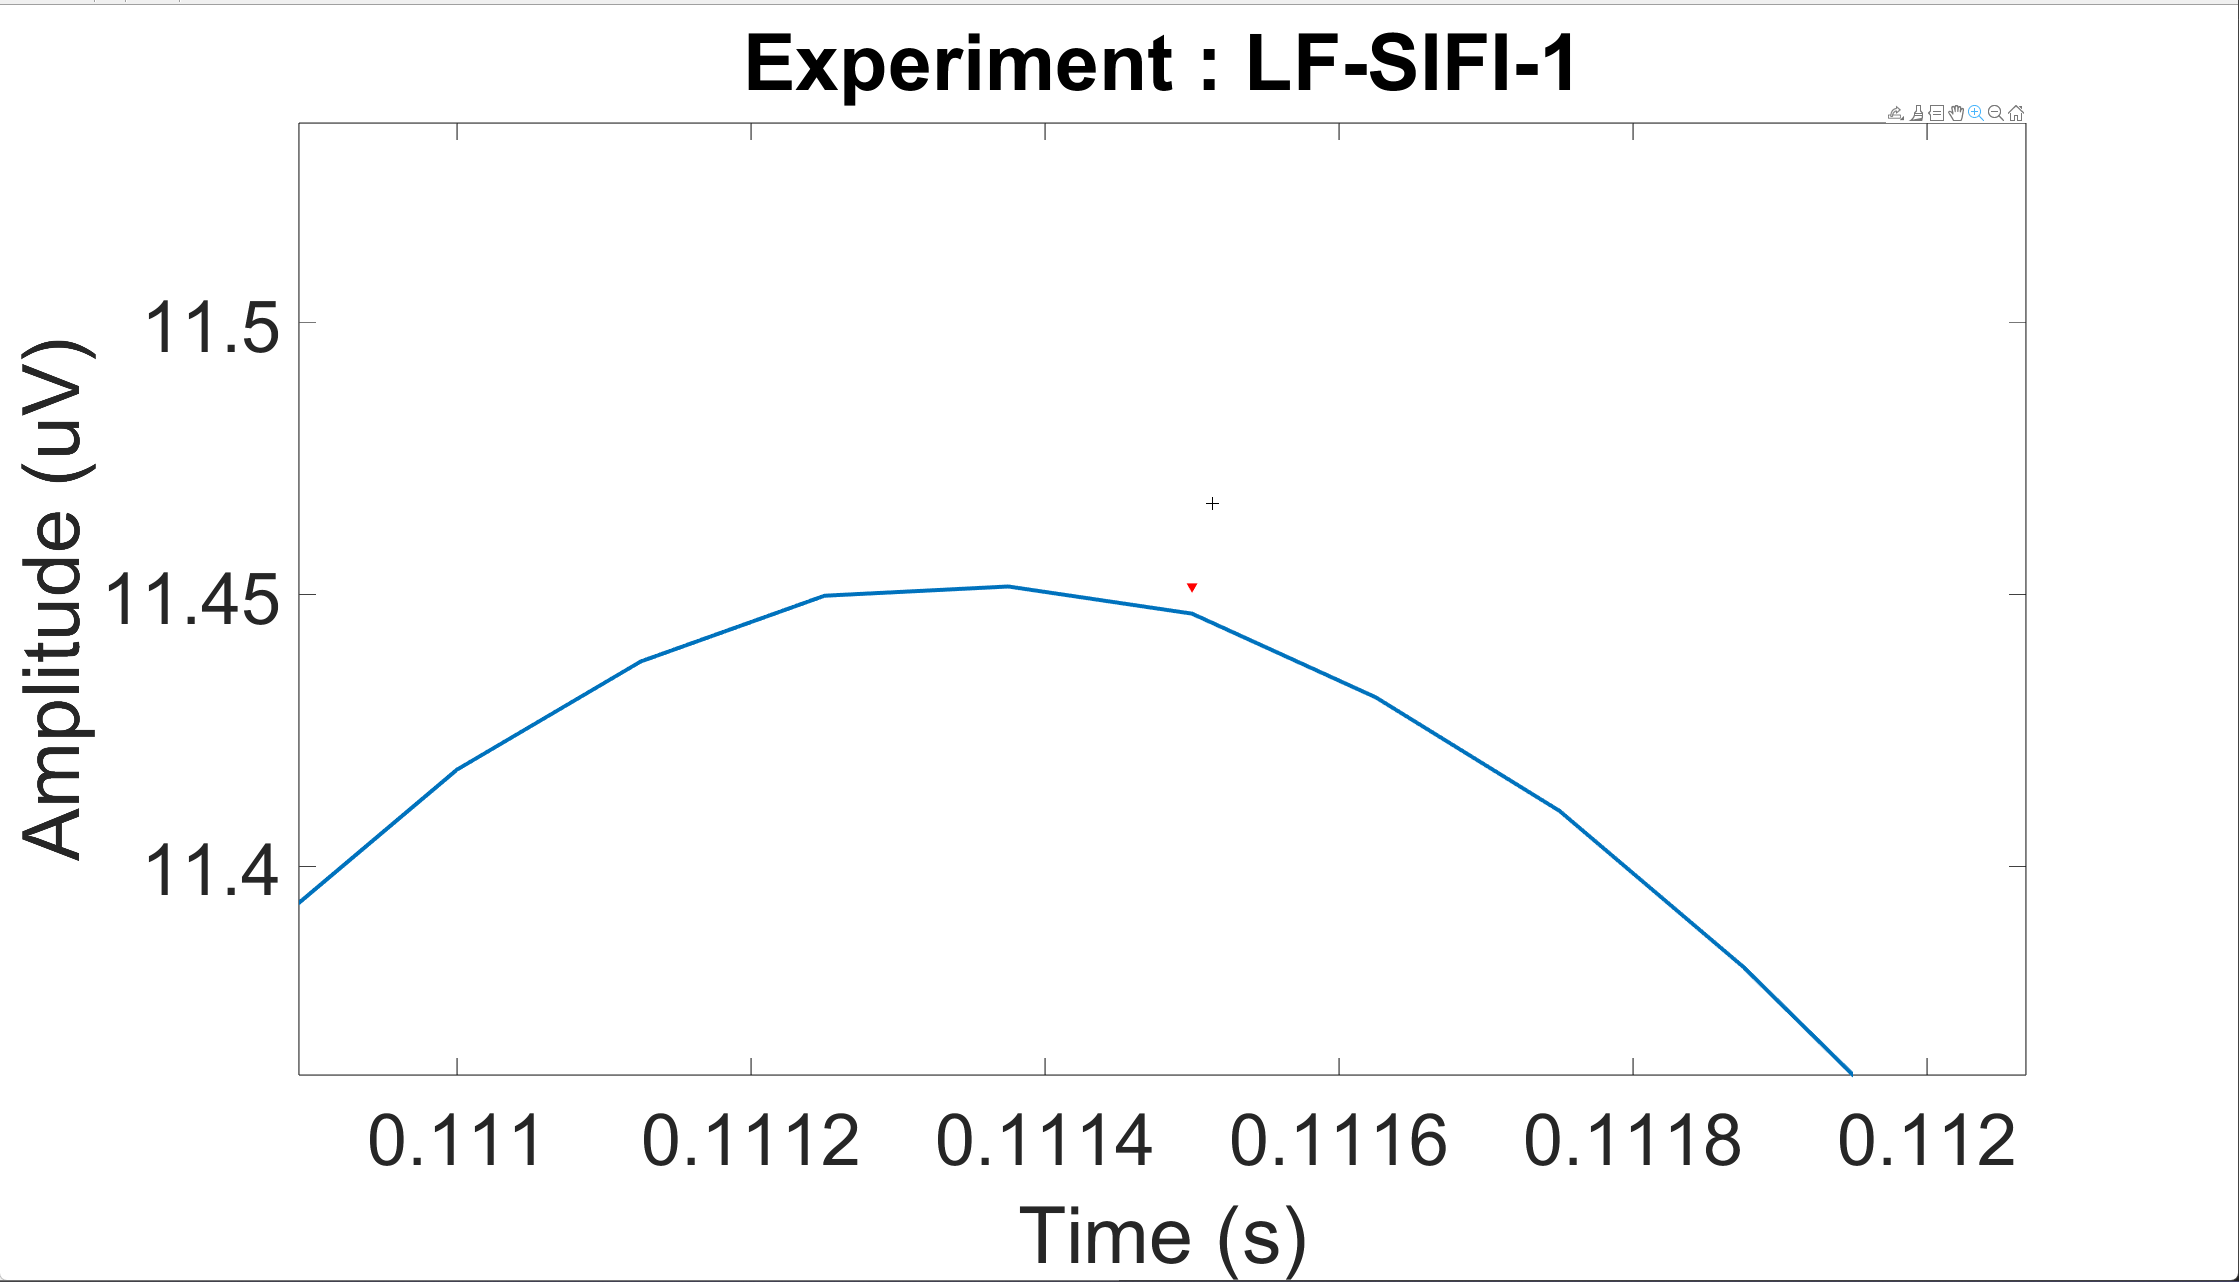
\includegraphics[scale=0.2]{"Images/LF-SIFI-1_Plot_Error.png"}
		\caption{P100 Label Error | LF-SIFI-1 (Dataset)}
	\end{figure}
	
	\begin{figure}[tbh!]\label{LF-SIFI-1-ErrorFix}
		\centering
		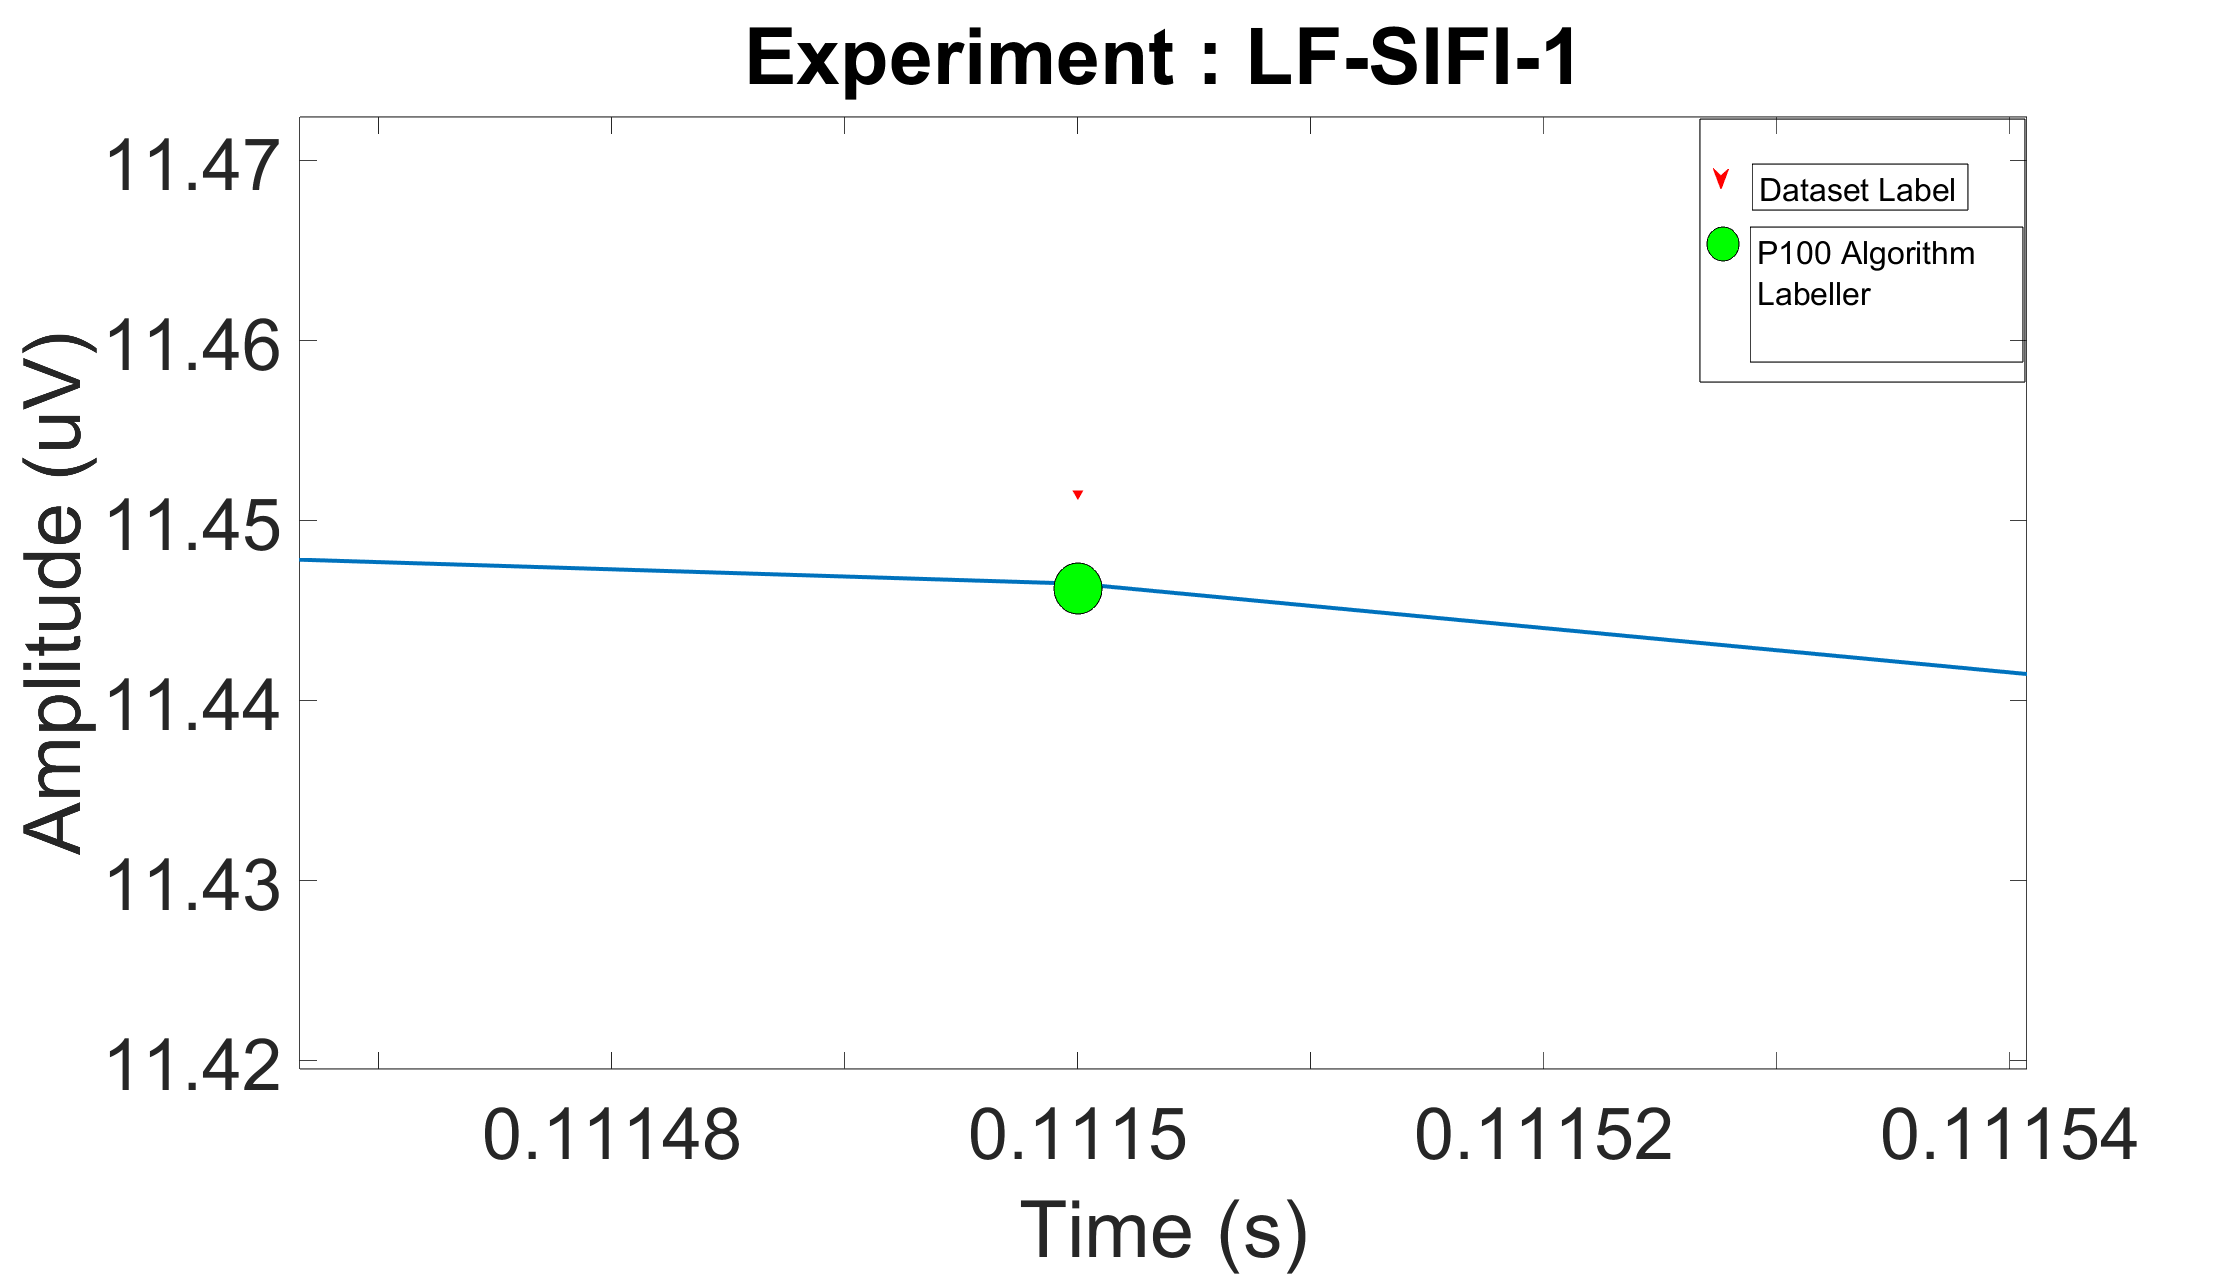
\includegraphics[scale=0.2]{"Images/LF-SIFI-1_Plot_ErrorFix.png"}
		\caption{P100 Labelling (Algorithm vs Dataset) | LF-SIFI-1}
	\end{figure}
	
		
	\begin{table}
		\centering
		\caption{Time Window (post stimulus) for Visually Evoked Potentials}
		\begin{tblr}{
				vline{1,2,3} = {-}{},
				hline{1,8} = {-}{0.08em},
				hline{2,3,4,5,6,7,8} = {-}{},
			}
			VEPs  & Time Window (Post Stimulus)\\                                            
			N35  & 35 ms\\                       
			P50  & 45-60 ms\\                                          
			N75 & 75 ms\\
			P100 & 80-130 ms\\
			N170 & 170 ms \\
			P200 & 180-250 ms \\
		\end{tblr}
		\label{tbl:VEP_TimeWindow}
	\end{table}
	
	\begin{table}
		\centering
		\caption{Time Window (post stimulus) for Auditory Evoked Potentials}
		\begin{tblr}{
				vline{1,2,3} = {-}{},
				hline{1,8} = {-}{0.08em},
				hline{2,3,4,5,6,7,8} = {-}{},
			}
			VEPs  & Time Window (Post Stimulus)\\                                            
			N0  & <50 ms\\                       
			P1  & 50-100 ms ms\\                                          
			N1 & 100 ms\\
			P2 & 150-200 ms\\
			N2 & 170-250 ms \\
			P3 & 250-500 ms \\
		\end{tblr}
		\label{tbl:AEP_TimeWindow}
	\end{table}
	
	
	
	
	\newpage
	\section{Conclusion}
	Since we cannot trust the validity of the dataset, new work has to be done to annotate the labels in a more strict fashion. We will then continue coming up with other algorithms but to determine the validity, we need an accurate version of the ground truth. 
	
	
	
	


	
	
	

\newpage
	
	
	% ------------------------------------------------------------------------------
	% Reference and Cited Works
	% ------------------------------------------------------------------------------
	
	\bibliographystyle{IEEEtran}
	\bibliography{References.bib}
	
	% ------------------------------------------------------------------------------
	
\end{document}